\documentclass[12pt, a4paper]{article}

%package
\usepackage[utf8]{inputenc}
\usepackage{amsmath} %For both in-line and equation mode
\numberwithin{equation}{section} %Numbering of our equations per section
\usepackage{algorithm}
\usepackage{algorithmic} %Algorithm styles, need to be nested for the example shown
\usepackage{fancyhdr} %For our headers
\usepackage{graphicx} %Inserting images
\usepackage{lipsum}  %Blank text fill, delete me when finished
\usepackage{setspace} %Spacing on the front page for crest and titles
\usepackage[]{fncychap} % Styles can be Sonny, Lenny, Glenn, Conny, Rejne, Bjarne and Bjornstrup
\usepackage[hyphens]{url} %Deals with hyphens in urls to make them clickable
\usepackage{xcolor} %Great if you want coloured text
\usepackage{tabularx}
\usepackage{appendix} %Take a wild guess slick

\fancyhf{}
\pagestyle{fancy}

\graphicspath{{../diagrams/images/}{../diagrams/images/png/}}

\title{Progetto Ingegneria del Software}
\author{Davide Bleggi \and Joshua Chapman}
\date{Giugno 2020}


\begin{document}
\begin{titlepage}
  \maketitle
\end{titlepage}

\begin{abstract}
  Progetto per la creazione di un sistema informatico per gestire il servizio 
  di spesa on-line di un supermercato.
\end{abstract}

<<<<<<< HEAD
% Table of content
\tableofcontents
\newpage

\section{Introduzione}
=======
>>>>>>> dev

% Table of content
\tableofcontents
\newpage


\section{Introduzione}
% Subsection divisione del lavoro, tentativo di scrum, e difficoltà della distanza
% Paired developement
Date le distanze, i tempi ristretti, e il nostro team composto da sole due persone abbiamo preferito usare al \textbf{XP programming}, in grado di adattarsi meglio alle nostre esigenze, e appoggiandoci ad un servizio di \textbf{Version Control System} quale \textbf{GIT} per poter proseguire anche in autonomia e non solo con l'ausilio del \textbf{pair programming}. Quindi durante la progettazione è stato tenuto un approccio \textbf{Test First Developement} seguito da costanti aggiornamenti di \textbf{refactoring}.

\subsection{Analisi Dei Requisiti}
% Cominciato con analisi dei requisiti, sezioni del pdf
% Backlog dei requisiti
Prima di tutto abbiamo cominciato con l'analisi dei requisiti forniti dalla documentazione. Quindi abbiamo estrapolato 6 macrosezioni principali:
\begin{itemize}
\item Registrazione
	\begin{itemize}
	\item Gli  utenti devono  essere  registrati.
	\item Ogni utente registrato accede con email e password.
	\item Gli utenti possono specificare un metodo di pagamento preferito.
	\end{itemize}
\item Catalogo
	\begin{itemize}
	\item  Se un utente inserisce un prodotto che al momento della conferma della spesa non risulta più disponibile,il sistema segnala la cosa al cliente ed elimina il prodotto dal carrello.
	\item Ogni utente registrato accede con email e password.
	\item Gli utenti possono specificare un metodo di pagamento preferito.
	\item Dopo aver confermato la spesa, l’utente sceglie data e orario della consegna visualizzando le opzioni possibili.
	\end{itemize}
\item Carrello
	\begin{itemize}
	\item L’utente può visualizzare il carrello per modificare la quantità dei prodotti inseriti o rimuovere qualche prodotto.
	\item L’utente può ricercare i prodotti per tipo (uova, biscotti, pasta), per marca o per eventuali caratteristiche.
	\end{itemize}
\item Effettua spesa
	\begin{itemize}
	\item  Ad ogni spesa vengono accreditati sulla tessera fedeltà un numero di punti pari agli euro spesi nella spesa considerata.
	\end{itemize}
\item Profilo utente
	\begin{itemize}
	\item  Il  sistema  deve  permettere  agli  utenti  di  accedere  al  loro  profilo,  modificare  i  dati  anagrafici, verificare il saldo punti e lo stato delle loro spese.
	\item Ogni utente può vedere tutte le spese che ha effettuato nel tempo con il dettaglio dei prodotti acquistati.
	\end{itemize}
\item Responsabili reparto
	\begin{itemize}
	\item  Il  sistema  deve  permettere  agli  utenti  di  accedere  al  loro  profilo,  modificare  i  dati  anagrafici, verificare il saldo punti e lo stato delle loro spese.
	\item Ogni utente può vedere tutte le spese che ha effettuato nel tempo con il dettaglio dei prodotti acquistati.
	\item I responsabili del reparto spesa on-line devono autenticarsi per poter accedere al sistema e devono poter  verificare  lo  stato delle  spese  e  provvedere  all’inserimento delle  informazioni  relative  ai prodotti.
	\end{itemize}
\end{itemize}
	

% Subsection framework e librerie usati spring per il server e okhttp3. Javafx
% build system gradle
\subsection{Framework}
Per il progetto si sono ritenuti necessarie una serie di implementazioni di librerie esterne.
\subsubsection{Spring}
Abbiamo utilizzato Spring (by Netfix) per un rapido sciluppo di un server compatibile con Java.
\subsubsection{Okhttp3}
Per la comunicazione tra client e Server, abbiamo optato per un libreria in grado di gestire le richieste http per creare una web application.
\subsubsection{JavaSQL}
Per la gestione del database javaSQL con il driver di SQLite.
\subsubsection{JavaFX}
Per l'interfaccia grafica è stato utilizzato JavaFX. Scelta perchè è il più moderno e permette di essere utilizzato senza ausilio di librerie esterne.
\subsubsection{Gradle}
Utilizzato per la Build System modulare e pers facilitare la compilazione cross-platform (importando automaticamente le librerie necessarie).

\section{Use Cases}

Nel sistema abbiamo identificato 8 use cases. Gli attori necessari per il 
sistema sono i seguenti:
\begin{itemize}
  \item Clienti
  \item Responsabili Reparto
  \item Utente
\end{itemize}

\begin{figure}[h]
\centering
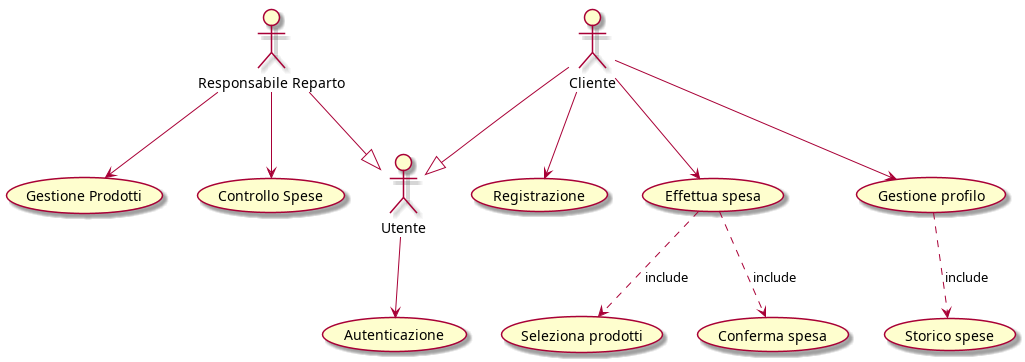
\includegraphics[width=\textwidth]{use_case_diagram.png}
\caption{Use case diagram}
\end{figure}

I due attori Cliente e Responsabile Reparto sono generalizzati nel attore Utente
per tutti gli use case di autenticazione, in quanto andranno ad autenticarsi
nello stesso portale.  Gli use case possono essere raggruppati in base 
all'attore a cui appartengono. Le funzioni principali del responsabile reparto 
sono di gestire prodotti e lo stato delle spese; gli use case del cliente sono
di registrarsi alla piattaforma, effettuare spese e gestire il proprio profilo.

\newpage

\subsection{User Use Cases}

Le seguenti sono gli use case del utente con i corrispettivi sequence diagrams.

\subsubsection{Autenticazione}

\begin{figure}[h]
\centering
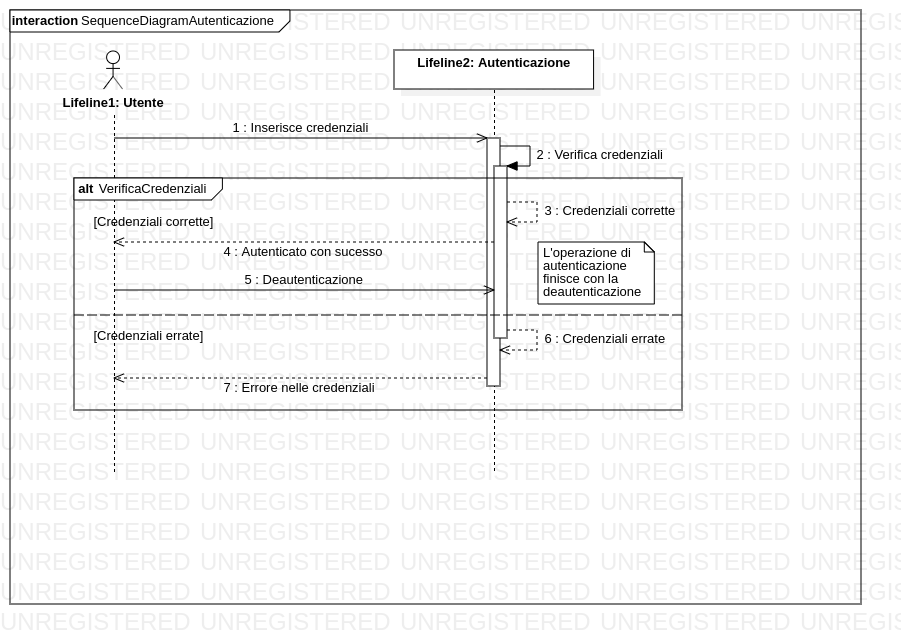
\includegraphics[width=\textwidth]{Use Case Model!Autenticazione!InteractionAutenticazione!SequenceDiagramAutenticazione_7.png}
\caption{Sequence diagram autenticazione}
\end{figure}

Quando l'utente deve autenticarsi, inserisce le credenziali nel portale. Queste
verranno verificate. Nel caso siano corrette verrà autenticato con successo, e 
potrà successivamente compiere il logout. Nel caso siano incorrette verrà
restituito un errore.

\newpage

\subsection{Responsabile Use Cases}

Le seguenti sono gli use case del responsabile del reparto con i corrispettivi 
sequence diagrams.

\subsubsection{Gestione Prodotti}

\begin{figure}[h]
\centering

\includegraphics[width=\textwidth]{Use Case Model!Gestione prodotti!InteractionGestioneProdotti!SequenceDiagramGestioneProdotto_9.png}
\caption{Sequence diagram gestione prodotti}
\end{figure}

\subsubsection{Controllo Spese}

\begin{figure}[h]
\centering
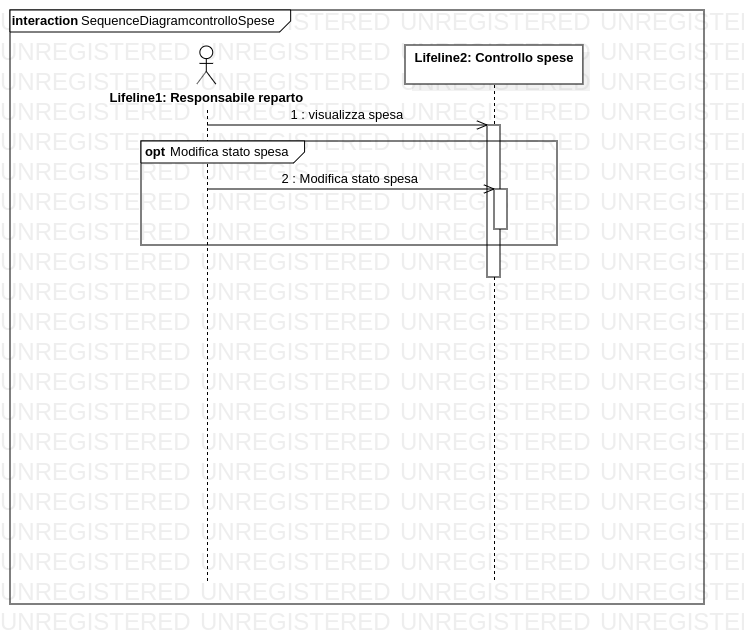
\includegraphics[width=\textwidth]{Use Case Model!Controllo spese!InteractionConstrolloSpese!SequenceDiagramcontrolloSpese_11.png}
\caption{Sequence diagram registrazione}
\end{figure}

\subsection{Client Use Cases}

Le seguenti sono gli use case del cliente con i corrispettivi sequence diagrams.

\subsubsection{Registrazione}

\begin{figure}[h]
\centering
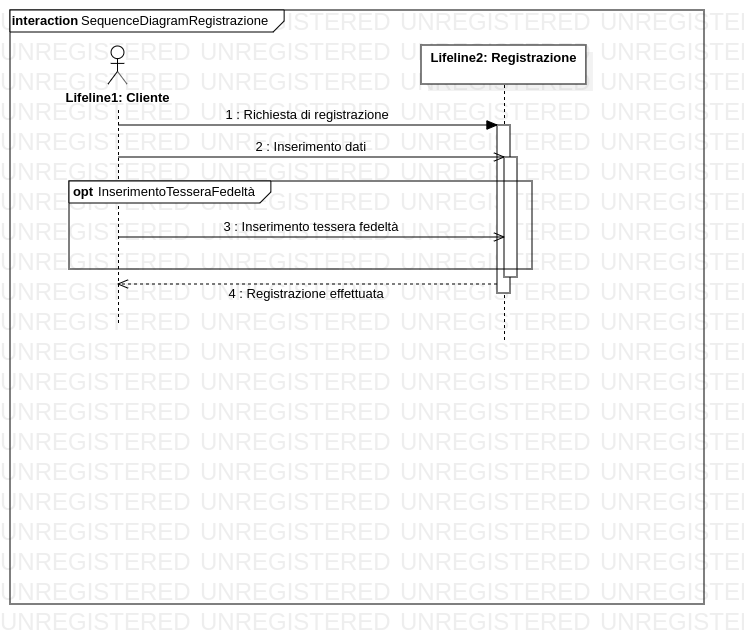
\includegraphics[width=\textwidth]{Use Case Model!Registrazione!InteractionRegistrazione!SequenceDiagramRegistrazione_1.png}
\caption{Sequence diagram registrazione}
\end{figure}

\subsubsection{Effettua Spesa}

\begin{figure}[h]
\centering
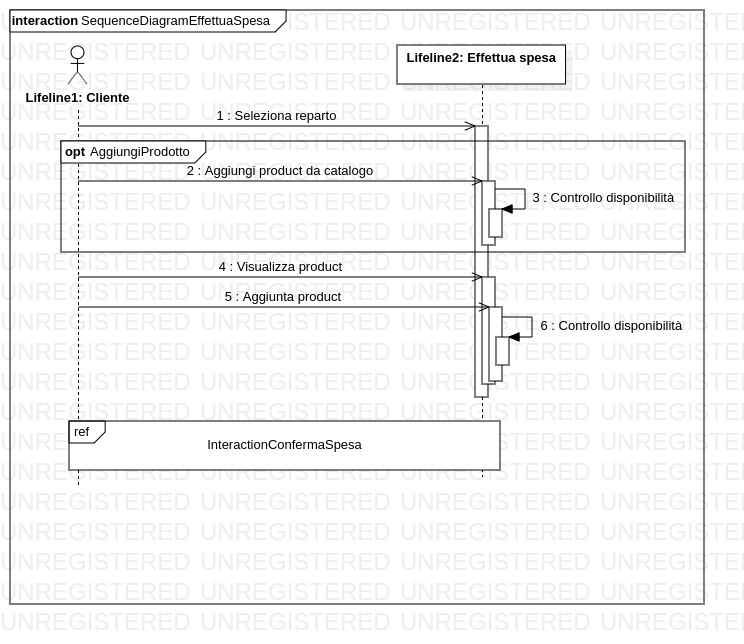
\includegraphics[width=\textwidth]{Use Case Model!Effettua spesa!InteractionEffettuaSpesa!SequenceDiagramEffettuaSpesa_3.png}
\caption{Sequence diagram registrazione}
\end{figure}

\begin{figure}[h]
\centering
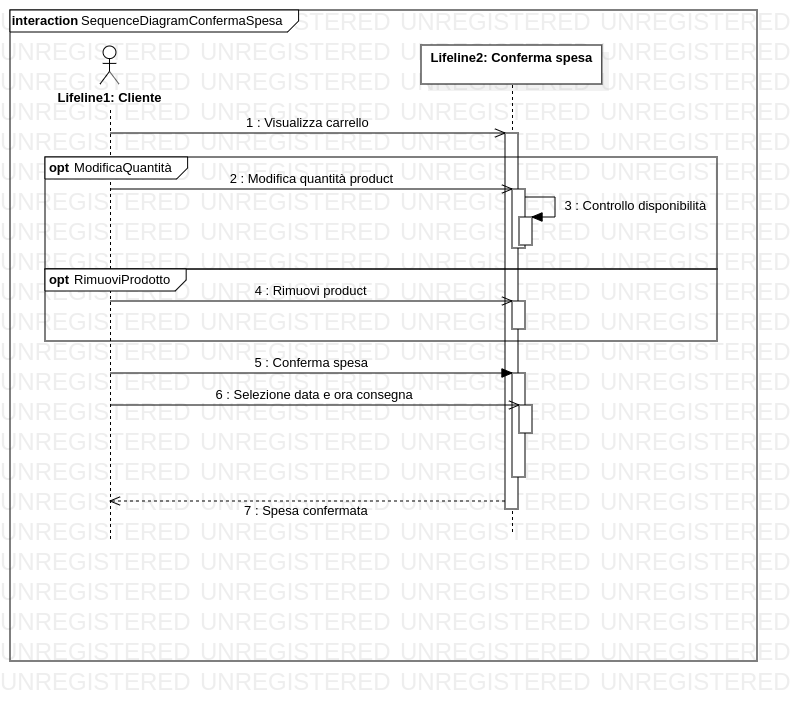
\includegraphics[width=\textwidth]{Use Case Model!Conferma spesa!InteractionConfermaSpesa!SequenceDiagramConfermaSpesa_13.png}
\caption{Sequence diagram registrazione}
\end{figure}

\subsubsection{Gestione Profilo}

\begin{figure}[h]
\centering
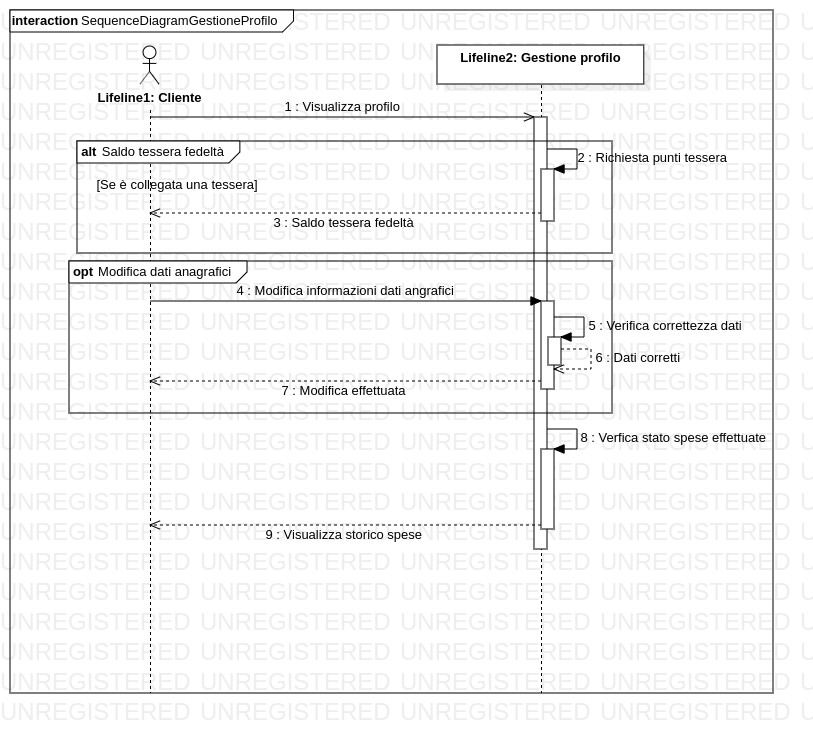
\includegraphics[width=\textwidth]{Use Case Model!Gestione profilo!InteractionGestioneProfilo!SequenceDiagramGestioneProfilo_5.png}
\caption{Sequence diagram registrazione}
\end{figure}

\section{Activity diagram}

% Activity diagram e spiegazione

\section{Pattern architetturali}

% MVC Server Repository(Database)

\section{Class diagram}

% Riassunto enf. classi più importanti
% Mod nel database simi modl client non ug

% Sezione server Router

% Sezione model Database
%   model Client

% Classe della Sessione
%   con eventuali robe

% Controllers
% Tutte sequence diagram

% Tasks & Components

\section{Discussione design patterns}

% Singletons
%   Database
%   Sessione
% DAO Observable Sessione
% Factory
%   Utente
% Gli altri non sono factory, ma li abbiamo tenuti cosi per divisione del codice
% e possibile ottimizzazione

\section{Test suite}

% TDD crea test, crea funzione intellij genera metodi
% Unit test tutto server, code coverage
% Javafx non testabile, ma funzioni attorno si
% CI/CD GitHub test automatici

\section{Conclusione}
Il progetto è stato condotto cercando inizialmente di rispettare le metodologia \textbf{Scrum} e utilizzando un \textbf{System Version Control} quale GIT per poter gestire al meglio il lavoro a distanza sullo stesso progetto. Dopo aver concordato degli sprint molto ristretti (una settimana circa) e avendo un brief ogni due giorni invece che 1, abbiamo cominciato col progetto.
% Pace e amore schifo java e javafx (╯°□°)╯︵ ┻━┻

\end{document}
